\section{여정의 시각화}

데이터는 보이지 않는다. 서버에 쌓이는 로그는 시간, 접속 IP, 행위의 기록(Log)일 뿐, 그 자체로는 아무런 서사도 보여주지 않는다. 앞서 설계한 온톨로지가 \enquote{지식의 지도}라면, 여정의 시각화(Visualization of Journey)는 그 지도 위에서 실제로 움직이는 \texttt{데이터의 흐름(Flow)}을 검증하는 과정이다.

시각화는 단순히 \enquote{결과를 보여주는 보고서}가 아니다. 온톨로지 관점에서 시각화는 \texttt{데이터 로직의 유닛 테스트(Unit Test for Data Logic)}와 같다. 이는 눈에 보이지 않는 데이터의 연결이 논리적으로 타당한지, 끊어진 곳은 없는지, 설계된 인과관계가 실제 데이터로 증명되는지를 확인하는 논리적 검증 수단이다.

\textbf{정적 스냅샷에서 동적 시퀀스로}

데이터베이스(DB)의 테이블은 \texttt{스냅샷(Snapshot)}이다. \enquote{특정 고객이 특정 시점에 상품을 구매했다}는 사실은 테이블의 한 행(Row)으로 기록된다. 하지만 이것만으로는 데이터 간의 인과관계를 설명할 수 없다. 온톨로지 기반의 시각화는 이 정적인 스냅샷들을 \texttt{시간의 축} 위에서 연결하여 하나의 \texttt{시퀀스(Sequence)}로 변환하는 작업이다.

\begin{itemize}
    \item \texttt{기존의 테이블 뷰}: 사용자(User), 주문(Order), 로그(Log) 테이블이 물리적으로 분리되어 있다. \enquote{누가(Who)}와 \enquote{무엇을(What)}은 존재하지만, 이들이 필연적으로 연결되는지는 알 수 없다.
    \item \texttt{온톨로지 뷰}: \enquote{검색(Search) $\xrightarrow{cause}$ 상품 조회(View) $\xrightarrow{cause}$ 장바구니 담기(Add-to-Cart) $\xrightarrow{cause}$ 구매(Purchase)}라는 데이터의 인과적 흐름이 명시적인 화살표(Edge)로 시각화된다.
\end{itemize}

\begin{figure}[ht]
    \centering
    \resizebox{\linewidth}{!}{
    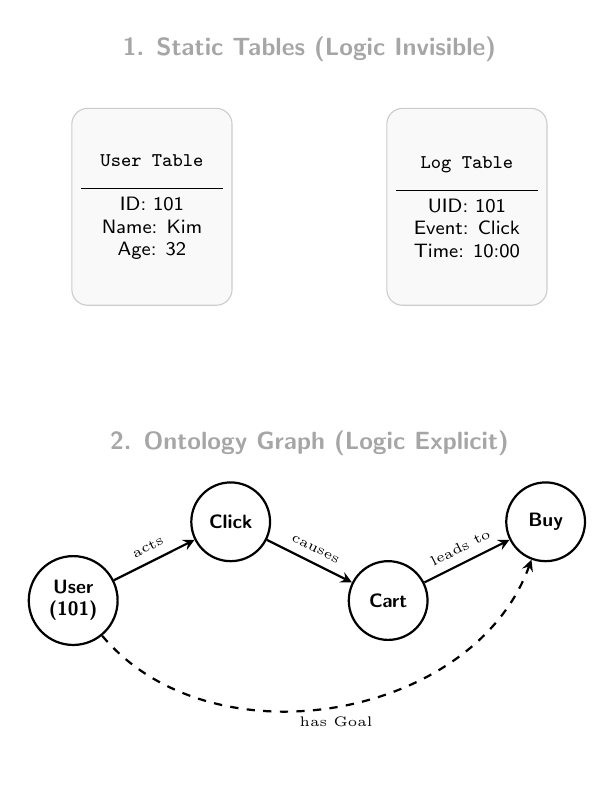
\begin{tikzpicture}[
        node distance=1.5cm,
        table/.style={
            rectangle, 
            draw=gray!40, 
            fill=gray!5, 
            rounded corners=2mm, 
            minimum width=2cm, 
            minimum height=2.5cm, 
            align=center, 
            font=\sffamily\scriptsize
        },
        graphnode/.style={
            circle, 
            draw=black, 
            fill=white, 
            thick, 
            minimum size=1cm, 
            align=center, 
            font=\sffamily\bfseries\scriptsize
        },
        arrow/.style={
            ->, 
            >=stealth, 
            thick, 
            draw=black
        },
        label/.style={
            font=\sffamily\bfseries\small, 
            text=gray!70
        }
    ]

    % --- Part 1: Relational Tables (Static) ---
    \node[label] at (0, 0.5) {1. Static Tables (Logic Invisible)};
    
    \node[table] (user) at (-2, -1.5) {
        \texttt{User Table}\\
        \rule{1.8cm}{0.4pt}\\
        ID: 101\\
        Name: Kim\\
        Age: 32
    };
    
    \node[table] (log) at (2, -1.5) {
        \texttt{Log Table}\\
        \rule{1.8cm}{0.4pt}\\
        UID: 101\\
        Event: Click\\
        Time: 10:00
    };
    
    % --- Part 2: Ontology Graph (Dynamic) ---
    \node[label] at (0, -4.5) {2. Ontology Graph (Logic Explicit)};
    
    \node[graphnode] (u) at (-3, -6.5) {User\\(101)};
    \node[graphnode] (e1) at (-1, -5.5) {Click};
    \node[graphnode] (e2) at (1, -6.5) {Cart};
    \node[graphnode] (e3) at (3, -5.5) {Buy};
    
    % Relationships
    \draw[arrow] (u) -- node[above, sloped, font=\tiny] {acts} (e1);
    \draw[arrow] (e1) -- node[above, sloped, font=\tiny] {causes} (e2);
    \draw[arrow] (e2) -- node[above, sloped, font=\tiny] {leads to} (e3);
    \draw[arrow, dashed, bend right=60] (u) to node[below, font=\tiny] {has Goal} (e3);

    \end{tikzpicture}
    }
    \caption[데이터의 관점 변화: 정적 테이블에서 동적 여정으로]{데이터의 관점 변화: 정적 테이블에서 동적 여정으로. 테이블 구조에서는 알 수 없는 인과관계가 온톨로지 그래프에서는 명시적인 화살표(Edge)로 드러난다.}
    \labfig{table_vs_graph}
\end{figure}

이러한 시각화는 단순히 \enquote{구매가 발생했다}는 결과뿐만 아니라, 그 결과에 도달하기까지의 과정을 \texttt{동적(Dynamic)}으로 보여준다. 만약 시각화된 여정에서 \enquote{장바구니 담기}와 \enquote{구매} 사이의 화살표가 빈번하게 끊어져 있다면, 그것은 단순한 이탈이 아니라 시스템 내 데이터 흐름의 단절을 의미한다.

\textbf{논리적 정합성의 검증}

데이터를 시각화한다는 것은 곧 \texttt{데이터 연결(Edge)의 진실성}을 확인하는 과정이다. \enquote{데이터 기반 의사결정}이 유효하려면, 그 기반이 되는 데이터의 연결 구조가 참(True)이어야 한다.

온톨로지로 시각화된 여정 지도는 전체 데이터 시스템에 대한 \texttt{단일한 논리적 뷰(Unified Logical View)}를 제공한다. \enquote{캠페인 반응 데이터}와 \enquote{구매 전환 데이터}는 별개의 사일로(Silo)에 존재하는 것이 아니라, 하나의 긴 인과 사슬(Causal Chain) 속에서 연결되어야만 한다.

이 과정에서 검증해야 할 핵심 질문은 \enquote{논리적으로 연결되어 있는가?}이다. 시각화 도구 위에서 데이터의 흐름이 끊김 없이 이어진다면, 온톨로지 모델링은 유효한 것이다. 반대로 여정이 끊겨서 보인다면, 그것은 데이터가 파편화되어 있다는 증거다. 결국 시각화는 데이터 통합의 완전성을 증명하는 성적표이자, 데이터 품질을 관리하는 모니터링 수단이 된다.

모든 데이터는 연결되어야 비로소 정보가 되고, 흐름이 되어야 통찰이 된다. 여정의 시각화는 그 흐름을 드러내어, 데이터가 단순한 적재물이 아니라 논리적인 서사를 가진 구조임을 증명한다.
